\documentclass[report.tex]{subfiles}
\begin{document}

\chapter{Excercise 0: Double mass-spring-damper system analysis}
\section{Diff. analysis}

For exercise 0 a double mass-spring-damper system has to be analysed

\begin{figure}[H]
	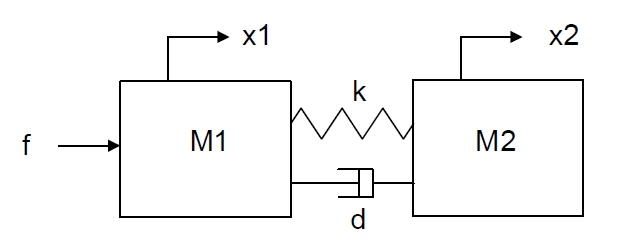
\includegraphics[width=0.8\textwidth]{msd_system}
	\centering
	\caption{A double mass-spring-damper system}
	\label{fig:intro_system}
\end{figure}
first the differential equations were deduced.\\

\begin{equation}
\label{eq:diffm1}
{ m }_{ 1 }{ \ddot { x }  }_{ 1 }=({ \dot { x }  }_{ 2 }-\dot { x } _{ 1 })d+({ x }_{ 2 }-{ x }_{ 1 })k+F
\end{equation}

\begin{equation}
\label{eq:diffm2}
{ m }_{ 2 }{ \ddot { x }  }_{ 2 }=({ \dot { x }  }_{ 1 }-\dot { x } _{ 2 })d+({ x }_{ 1 }-{ x }_{ 2 })k
\end{equation}
in \eqref{eq:diffm1} the differential equation of the first mass is deduced, with on the left hand side the inertia of the mass and on the right hand the forces acting on M1.\\
the same holds for \eqref{eq:diffm2}\\
\\
\section{Transfer functions}
next the transfer function ${ H }_{ 1 }(s)=\frac { { X }_{ 1 }(s) }{ F(s) } $ are to be defined. first the laplace transfer of both \eqref{eq:diffm1} and \eqref{eq:diffm2} are defined, and rewritten to $x_1=...$ and $x_2=...$\\
\\

\begin{equation}
\label{eq:lap_x1}
x_1=\frac{x_2(ds+k)+F}{M_1s^2+ds+k}
\end{equation}
\begin{equation}
\label{eq:lap_x2}
x_2=\frac{x_1(ds+k)+F}{M_2s^2+ds+k}
\end{equation}

the problem is simplified by assuming $M_1=M_2=M$ with use of substitution x2 is eliminated from \eqref{eq:lap_x1}

\begin{equation}
\label{eq:H1_1}
x_1=\frac{x_1(ds+k)+F}{M_2s^2+ds+k}\cdot\frac{(ds+k)+F}{M_1s^2+ds+k}
\end{equation}
Assuming $M_1=M_2=M$ and simplifying \eqref{eq:H1_1} results in.

\begin{equation}
\label{eq:H1_2}
H_1=\frac{x_1}{F}=\frac{Ms^2+ds+k}{s^2(s^2M^2+2Mds+2Mk)}
\end{equation}

next the trasnfer function ${ H }_{ 2 }(s)=\frac { { X }_{ 2 }(s) }{ F(s) } $ is deduced and results in
\begin{equation}
\label{eq:H2}
H_2=\frac{x_2}{F}=\frac{ds+k}{s^2(s^2M^2+2Mds+2Mk)}
\end{equation}
\section{Bode plot}
now to finish the analysis a bode plot is made.
first to to this the poles and zero's have to be determined of the system
both the transfer functions have the same denominators and resulting in the same poles

first the poles:
\begin{equation}
s^2(s^2M^2+2Mds+2Mk)=0
\end{equation}
this gives that there are 2 poles on s=0
next the abc formula is used to compute the other poles resulting in
\begin{equation}
s=\frac{-d\pm\sqrt{d^-4Mk}}{M}
\end{equation}
these are most likely 2 imaginary poles (the spring will have more force then the damper) with negative real parts\\
next are the zero's of the system first $H_1$ is deduced
\begin{equation}
Ms^2+ds+k=0
\end{equation}
using the abc-formula gives
\begin{equation}
s=\frac{-d\pm\sqrt{\frac{1}{4}d^-Mk}}{2M}
\end{equation}
so $H_1$ has 2 zero's and again it is likely that both are imaginary numbers with negative real parts\\
next are the zero' of $H_2$

\begin{equation}
ds+k=0
\end{equation}
\begin{equation}
s=-\frac{k}{d}
\end{equation}

\end{document}


